\iffalse

INSTRUCTIONS: (if this is not lecture1.tex, use the right file name)

  Clip out the ********* INSERT HERE ********* bits below and insert
appropriate TeX code.  Once you are done with your file, run

  ``latex lecture1.tex''

from a UNIX prompt.  If your LaTeX code is clean, the latex will exit
back to a prompt.  Once this is done, run

  ``dvips lecture1.dvi''

which should print your file to the nearest printer.  There will be
residual files called lecture1.log, lecture1.aux, and lecture1.dvi.
All these can be deleted, but do not delete lecture1.tex.
\fi
%
\documentclass[11pt]{article}
\usepackage{amsfonts}
\usepackage{amsmath}
\usepackage{latexsym}
\usepackage{hyperref}
\usepackage{multicol}
\usepackage{tikz}

\usepackage{tikz-qtree}
\usetikzlibrary{automata,arrows}

\hypersetup{
    colorlinks=true,
    linkcolor=blue,
    filecolor=magenta,      
    urlcolor=cyan,
}
 
\urlstyle{same}

\setlength{\oddsidemargin}{.25in}
\setlength{\evensidemargin}{.25in}
\setlength{\textwidth}{6in}
\setlength{\topmargin}{-0.4in}
\setlength{\textheight}{9.5in}

\newcommand{\handout}[5]{
   %\renewcommand{\thepage}{#1-\arabic{page}}
   \noindent
   \begin{center}
   \framebox{
      \vbox{
    \hbox to 5.78in { {\bf Data Structures and Algorithms} \hfill #2 }
       \vspace{4mm}
       \hbox to 5.78in { {\Large \hfill #5  \hfill} }
       \vspace{2mm}
       \hbox to 5.78in { {\it #3 \hfill #4} }
      }
   }
   \end{center}
   \vspace*{4mm}
}

\newcommand{\lecture}[3]{\handout{L#1}{#2}{}{}{#1}}

\def\squarebox#1{\hbox to #1{\hfill\vbox to #1{\vfill}}}
\def\qed{\hspace*{\fill}
        \vbox{\hrule\hbox{\vrule\squarebox{.667em}\vrule}\hrule}}
\newenvironment{solution}{\begin{trivlist}\item[]{\bf Solution:}}
                      {\qed \end{trivlist}}
\newenvironment{solsketch}{\begin{trivlist}\item[]{\bf Solution Sketch:}}
                      {\qed \end{trivlist}}
\newenvironment{proof}{\begin{trivlist}\item[]{\bf Proof:}}
                      {\qed \end{trivlist}}

\newtheorem{theorem}{Theorem}
\newtheorem{corollary}[theorem]{Corollary}
\newtheorem{lemma}[theorem]{Lemma}
\newtheorem{observation}[theorem]{Observation}
\newtheorem{remark}[theorem]{Remark}
\newtheorem{proposition}[theorem]{Proposition}
\newtheorem{definition}[theorem]{Definition}
\newtheorem{Assertion}[theorem]{Assertion}
\newtheorem{fact}[theorem]{Fact}
\newtheorem{hypothesis}[theorem]{Hypothesis}
%\newtheorem{observation}[theorem]{Observation}
%\newtheorem{proposition}[theorem]{Proposition}
\newtheorem{claim}[theorem]{Claim}
\newtheorem{assumption}[theorem]{Assumption}

%Put more macros here, as needed.
\newcommand{\al}{\alpha}
\newcommand{\Z}{\mathbb Z}
\newcommand{\jac}[2]{\left(\frac{#1}{#2}\right)}
\newcommand{\set}[1]{\{#1\}}

\def\ppt{{\sf PPT}}
\def\poly{{\sf poly}}
\def\negl{{\sf negl}}
\def\owf{{\sf OWF}}
\def\owp{{\sf OWP}}
\def\tdp{{\sf TDP}}
\def\prg{{\sf PRG}}
\def\prf{{\sf PRF}}

%end of macros
\begin{document}


\fbox{
\vbox{
\begin{flushleft}
Ann,  Bob, Charlie    (\emph{replace with your names})\\  % authors' names
COSC 336  \\  %class
3/19/2020   (\emph{replace with the current date})\\  % date
\end{flushleft}
\center{\Large{\textbf{Assignment 8}}}
%\end{mdframed}
} % end vbox
} % end fbox
\vline

\textbf{Instructions.}
\begin{enumerate}
\item Due  date announced on Blackboard.



\item This is a team assignment. Work in teams as in the previous assignments.  Submit one assignment per team, with the names of all students making the team.


\item Your programs must be written in Java.

\item Write your programs neatly - imagine yourself grading your program and see if it is easy to read and understand. 
At the very beginning present your algorithm in plain English or in pseudo-code (or both).
Comment your programs reasonably: there is no need to comment lines like "i++" but do include brief comments describing the main purpose of a specific block of lines.

\item  You will submit on Blackboard 2 files. The first file should be a .pdf file  with the solutions of the Exercise  and a  short description in English or in pseudocode of the algorithm for the  programming task  you are required to do and the results that you are required to report. Also include in this file, the Java code so that the grader can make comments.

Files 2 will contain the java code  for the programming   task.





%Staple all pages together.  You should have the electronic copy  of your programs with you (for example on a memory stick) because you may be asked to make a demo.

For editing the above document with  Latex, see the template posted on the course website. 
 
           assignment-template.tex	and
           
          assignment-template.pdf


To append in the  latex file  a pdf file, place it  in the same folder and then include them  in the latex file with 
\begin{verbatim}
\includepdf[pages=-,pagecommand={},width=\textwidth]{file.pdf}

\end{verbatim}
To append in the  latex file a .jpg file (for a photo), use 
\begin{verbatim}
\includegraphics[width=\linewidth]{file.jpg}

\end{verbatim}


\end{enumerate}
\newpage


\textbf{Exercise 1.}

We have seen that Dijkstra's algorithm can be implemented in two ways: Variant (a) uses an array to store the $dist[]$ values of the unknown nodes, and Variant (b) uses a MIN-HEAP to store these values.
\medskip

(a) Suppose in your application $m \le 3n$. Which variant gives a faster runtime?  Justify your answer.


(b) Suppose in your application $m \ge n^2/3$. Which variant gives a faster runtime?  Justify your answer.

(c) Suppose that your application $m = n^{3/2}$.   Which variant gives a faster runtime?  Justify your answer.

\bigskip


\textbf{Exercise 2.}   Recall that when we do DFS with timing every node $u$ gets 2 numbers that were denoted $u.d$ and $u.f$.   $u.d$ is the discovery time and $u.f$ is the finish time.   

Show that in a DAG (directed acyclic graph),  for any two nodes $u$ and $v$ such that there exists a path from $u$ to $v$, it holds that $u.f > v. f$.

Hint: There are two cases to analyze. Case 1 is that $u.d < v.d$ (in words, $u$ is discovered before $v$), and Case 2 is that $v.d < u.d$ (so, $v$ is discovered before $u$). In both cases, you need to argue that $u.f > v.f$.

\newpage
\textbf{Programming Task}

Write the program that modifies Breadth First Search  (see for example  the basic version of BFS in Notes 10) in such a way that given an undirected connected graph $G$, and a starting node $s$, it will print for every node $v$ the length of the shortest path from $s$ to $v$ and also the number of shortest paths from $s$ to $v$. Thus, you'll have two arrays $dist$ and $npath$, and for each vertex $v$, at the end of the program, $dist[v]$ will be equal to the length of a shortest path from $s$ to $v$ (like in the basic version of BFS), and $npath[v]$ will be equal to the number of shortest paths from $s$ to $v$.


For example, if $G_1$ is the first graph below, the length of a shortest path from 1 to 7 is 3, and there are three shortest paths from 1 to 7, namely 

1 - 2 - 5 - 7, 

1 - 3 - 5 - 7 and 

1 - 4 - 6 -7.

So,  $dist[7]=3$, and $npath[7] = 3$.
\medskip


Test your program on the graphs $G_1$ and $G_2$ (see the figures) using $1$ as the starting node. Your program is required to print the two arrays $dist[]$ and $npath[]$. Report the results you have obtained for these two graphs. 


You must use the adjacency list representation of a graph. As in the programming task from assignment 7, for the adjacency list, you \textbf{must} use the Java class \textsf{Adj\_List\_Graph} given in the file \textsf{Adj\_List\_Graph.java} (see \textsf{Test\_Adj.java} for a very simple example of using this class).  Note that, unlike Assignment 7,  in this  assignment you work with undirected graphs. So,   in \textsf{Adj\_List\_Graph.java}, you need to uncomment a line to make it work for undirected graphs.  
\bigskip

\begin{multicols}{2}

 graph $G_1$ 
\medskip



\begin{tikzpicture}[>=stealth',shorten >=1pt,auto,node distance=2.0cm,scale=0.3][h]
%\begin{tikzpicture}[shorten >=1pt,auto,node distance=2.8cm]][h]
  \node[state] (1) {$1$};
  \node[state] (2) [below left of =1] {$2$};
  \node[state] (3) [right of=2] {$3$};
  \node[state] (4) [right of=3] {$4$};
  \node[state] (5) [below of=2] {$5$};
\node[state] (6) [below of=4] {$6$};
\node[state] (7) [below of=5] {$7$};

  
  
  \path[-]
    (1) edge  (2)    
    (1) edge  (3) 
    (1) edge  (4) 
    (2) edge (5)
    (3) edge (5)
    (4) edge (6)
    (5) edge (6)
    (5) edge (7)
    (6) edge (7)
    ;
   
\end{tikzpicture}
%\bigskip

\columnbreak


graph $G_2$:
\medskip

 \begin{tikzpicture}[>=stealth',shorten >=1pt,auto,node distance=2.0cm,scale=0.3]][h]
%\begin{tikzpicture}[shorten >=1pt,auto,node distance=2.8cm]][h]
  \node[state] (1) {$1$};
  \node[state] (2) [below left of =1] {$2$};
  \node[state] (3) [right of=2] {$3$};
  \node[state] (4) [right of=3] {$4$};
  \node[state] (5) [right of=4] {$5$};
\node[state] (6) [right  of=5] {$6$};
\node[state] (7) [below of=4] {$7$};
\node[state] (8) [below left  of=7] {$8$};
\node[state] (9) [below right  of =7] {$9$};
\node[state](10)[below right of=8]{$10$};
  
  
  \path[-]
    (1) edge  (2)    
    (1) edge  (3) 
    (1) edge  (4) 
    (1) edge (5)
    (1) edge (6)
    (7) edge  (2)    
    (7) edge  (3) 
    (7) edge  (4) 
    (7) edge (5)
    (7) edge (6)
    (7) edge (8)
    (7) edge (9)
    (8) edge (10)
     (9) edge (10)
    ;
   
\end{tikzpicture}

\end{multicols} 
 
 
 \end{document}




\end{document}
